\documentclass{standalone}
\usepackage{tikz}
\usetikzlibrary{patterns, positioning}
\usepackage[sfdefault]{ClearSans} %% option 'sfdefault' activates Clear Sans as the default text font
\usepackage[T1]{fontenc}

\begin{document}
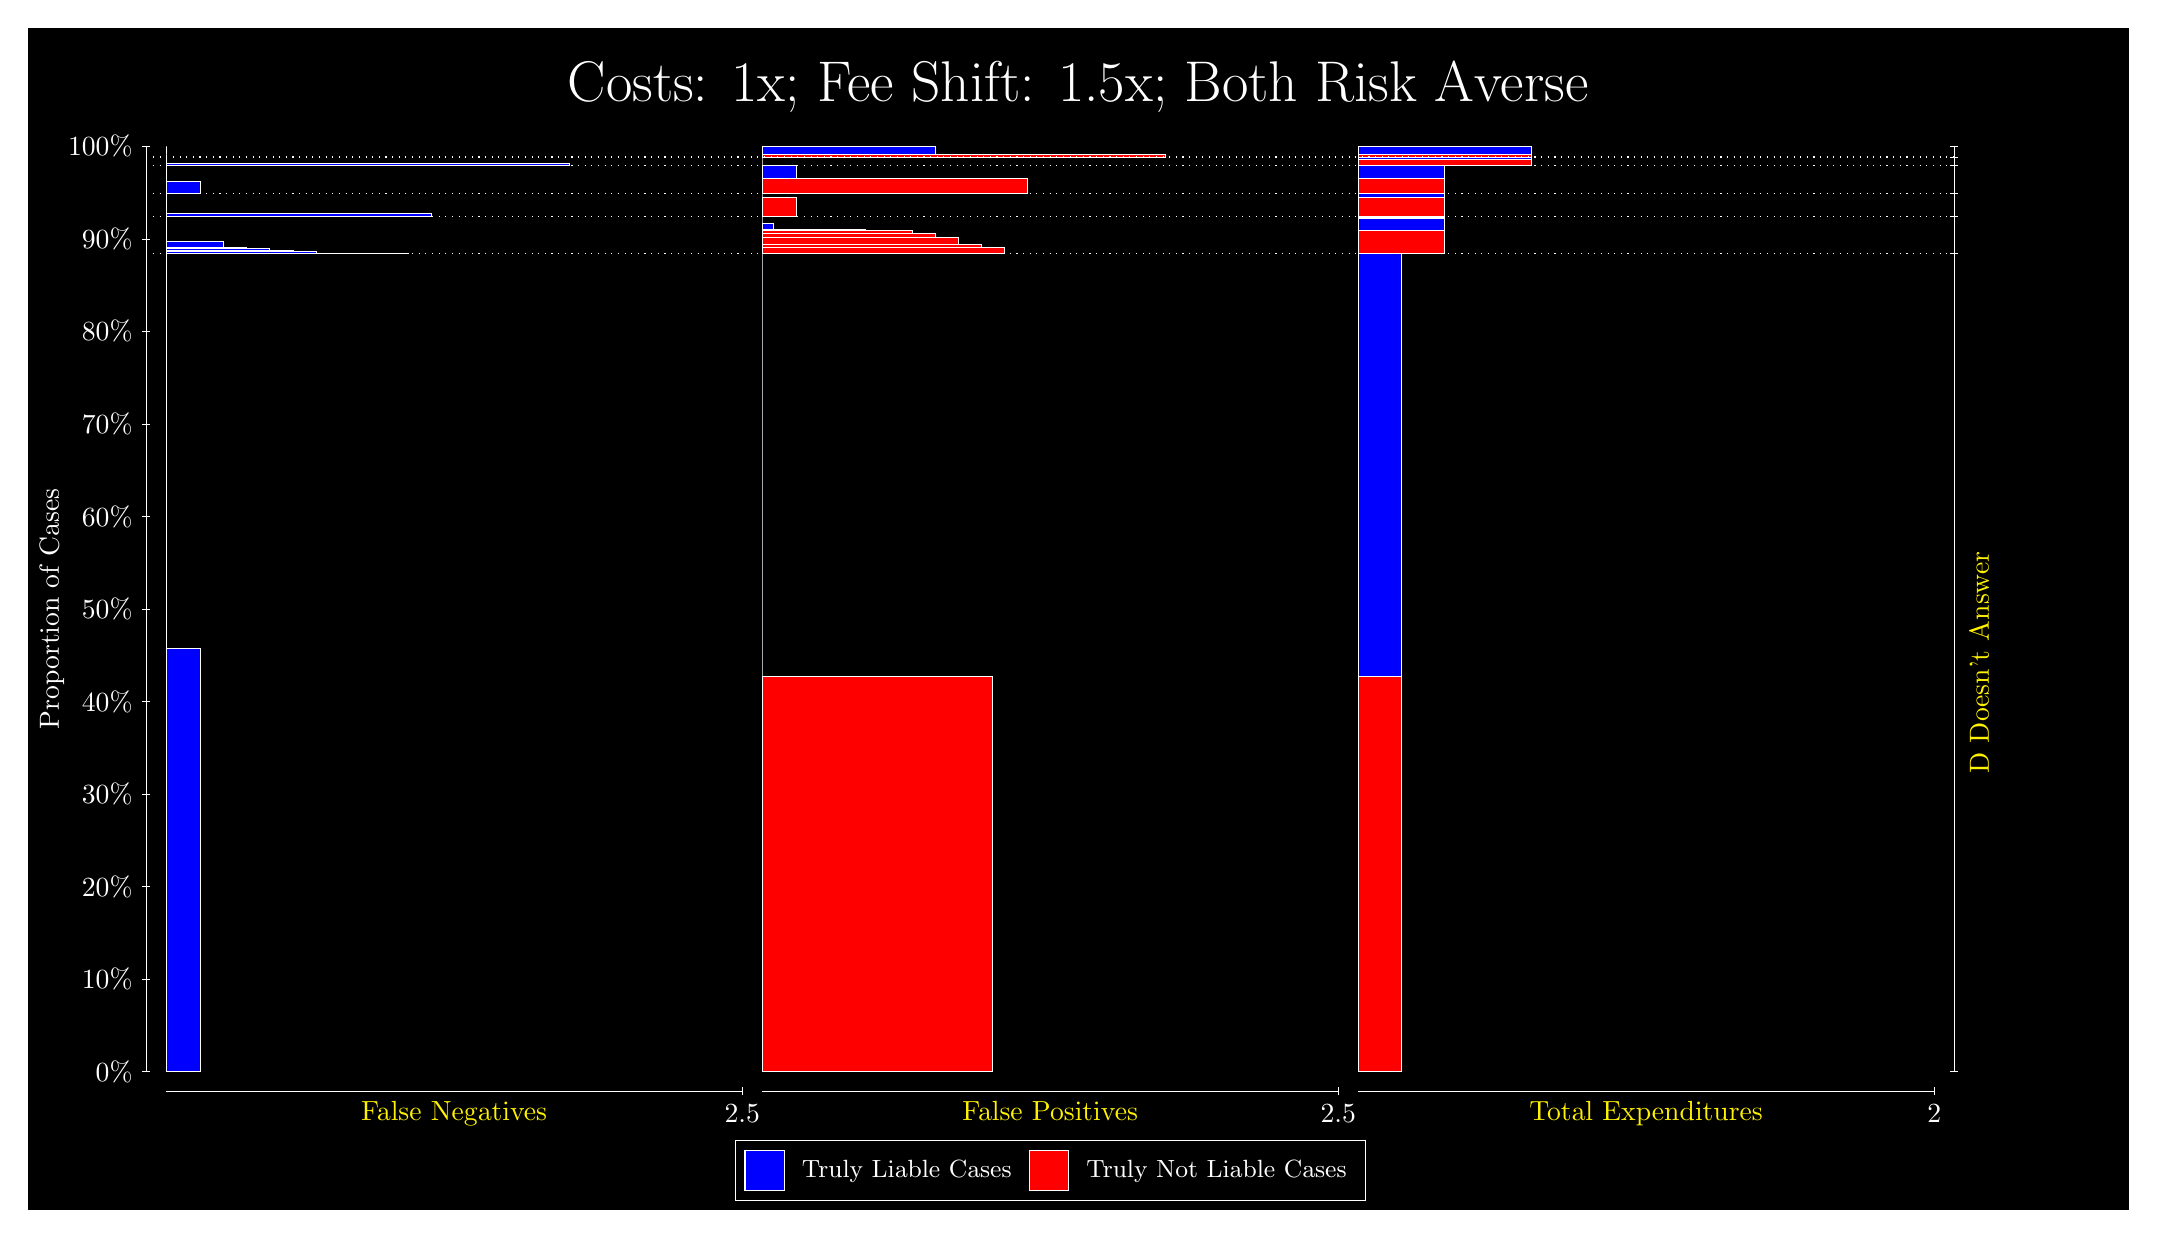
\begin{tikzpicture}
\draw[fill=black] (0,0) rectangle (26.667,15);
\draw[text=white] (0,13.5) rectangle (26.667,15) node[midway] {\huge Costs: 1x; Fee Shift: 1.5x; Both Risk Averse};
\draw[white, very thin] (1.5,1.75) -- (1.5,13.5);
\node[rotate=90, text=white, anchor=center] at (0.3, 7.625) {Proportion of Cases};
\draw[white, very thin] (1.45,1.75) -- (1.55,1.75);
\node[text=white, anchor=east] at (1.45, 1.75) {0\%};
\draw[white, very thin] (1.45,2.925) -- (1.55,2.925);
\node[text=white, anchor=east] at (1.45, 2.925) {10\%};
\draw[white, very thin] (1.45,4.1) -- (1.55,4.1);
\node[text=white, anchor=east] at (1.45, 4.1) {20\%};
\draw[white, very thin] (1.45,5.275) -- (1.55,5.275);
\node[text=white, anchor=east] at (1.45, 5.275) {30\%};
\draw[white, very thin] (1.45,6.45) -- (1.55,6.45);
\node[text=white, anchor=east] at (1.45, 6.45) {40\%};
\draw[white, very thin] (1.45,7.625) -- (1.55,7.625);
\node[text=white, anchor=east] at (1.45, 7.625) {50\%};
\draw[white, very thin] (1.45,8.8) -- (1.55,8.8);
\node[text=white, anchor=east] at (1.45, 8.8) {60\%};
\draw[white, very thin] (1.45,9.975) -- (1.55,9.975);
\node[text=white, anchor=east] at (1.45, 9.975) {70\%};
\draw[white, very thin] (1.45,11.15) -- (1.55,11.15);
\node[text=white, anchor=east] at (1.45, 11.15) {80\%};
\draw[white, very thin] (1.45,12.325) -- (1.55,12.325);
\node[text=white, anchor=east] at (1.45, 12.325) {90\%};
\draw[white, very thin] (1.45,13.5) -- (1.55,13.5);
\node[text=white, anchor=east] at (1.45, 13.5) {100\%};

\draw[white, very thin] (24.457,1.75) -- (24.457,13.5);
\draw[white, very thin] (24.407,1.75) -- (24.507,1.75);
\node[anchor=west] at (24.407, 1.75) {};
\draw[white, very thin] (24.407,12.138) -- (24.507,12.138);
\node[anchor=west] at (24.407, 12.138) {};
\draw[white, very thin] (24.407,12.607) -- (24.507,12.607);
\node[anchor=west] at (24.407, 12.607) {};
\draw[white, very thin] (24.407,12.898) -- (24.507,12.898);
\node[anchor=west] at (24.407, 12.898) {};
\draw[white, very thin] (24.407,13.257) -- (24.507,13.257);
\node[anchor=west] at (24.407, 13.257) {};
\draw[white, very thin] (24.407,13.365) -- (24.507,13.365);
\node[anchor=west] at (24.407, 13.365) {};
\draw[white, very thin] (24.407,13.5) -- (24.507,13.5);
\node[anchor=west] at (24.407, 13.5) {};

\draw[white, very thin, fill=blue] (1.75,1.75) rectangle (2.1891,7.1205);
\draw[white, very thin, fill=red] (1.75,7.1205) rectangle (1.75,12.138);
\draw[white, very thin, fill=blue] (1.75,12.138) rectangle (4.8239,12.14);
\draw[white, very thin, fill=blue] (1.75,12.14) rectangle (4.5312,12.141);
\draw[white, very thin, fill=blue] (1.75,12.141) rectangle (4.2384,12.144);
\draw[white, very thin, fill=blue] (1.75,12.144) rectangle (3.9457,12.148);
\draw[white, very thin, fill=blue] (1.75,12.148) rectangle (3.6529,12.161);
\draw[white, very thin, fill=blue] (1.75,12.161) rectangle (3.3602,12.175);
\draw[white, very thin, fill=blue] (1.75,12.175) rectangle (3.0674,12.204);
\draw[white, very thin, fill=blue] (1.75,12.204) rectangle (2.7746,12.222);
\draw[white, very thin, fill=blue] (1.75,12.222) rectangle (2.4819,12.298);
\draw[white, very thin, fill=red] (1.75,12.298) rectangle (1.75,12.607);
\draw[white, very thin, fill=blue] (1.75,12.607) rectangle (5.1167,12.655);
\draw[white, very thin, fill=red] (1.75,12.655) rectangle (1.75,12.898);
\draw[white, very thin, fill=blue] (1.75,12.898) rectangle (2.1891,13.06);
\draw[white, very thin, fill=red] (1.75,13.06) rectangle (1.75,13.257);
\draw[white, very thin, fill=blue] (1.75,13.257) rectangle (6.8732,13.289);
\draw[white, very thin, fill=red] (1.75,13.289) rectangle (1.75,13.365);
\draw[white, very thin, fill=red] (1.75,13.365) rectangle (1.75,13.397);
\draw[white, very thin, fill=blue] (1.75,13.397) rectangle (1.75,13.5);
\draw[white, very thin, fill=red] (9.3189,1.75) rectangle (12.246,6.7677);
\draw[white, very thin, fill=blue] (9.3189,6.7677) rectangle (9.3189,12.138);
\draw[white, very thin, fill=red] (9.3189,12.138) rectangle (12.393,12.22);
\draw[white, very thin, fill=red] (9.3189,12.22) rectangle (12.1,12.261);
\draw[white, very thin, fill=red] (9.3189,12.261) rectangle (11.807,12.346);
\draw[white, very thin, fill=red] (9.3189,12.346) rectangle (11.515,12.391);
\draw[white, very thin, fill=red] (9.3189,12.391) rectangle (11.222,12.431);
\draw[white, very thin, fill=red] (9.3189,12.431) rectangle (10.929,12.434);
\draw[white, very thin, fill=red] (9.3189,12.434) rectangle (10.929,12.437);
\draw[white, very thin, fill=red] (9.3189,12.437) rectangle (10.636,12.442);
\draw[white, very thin, fill=red] (9.3189,12.442) rectangle (10.344,12.444);
\draw[white, very thin, fill=red] (9.3189,12.444) rectangle (10.051,12.447);
\draw[white, very thin, fill=blue] (9.3189,12.447) rectangle (9.4652,12.523);
\draw[white, very thin, fill=blue] (9.3189,12.523) rectangle (9.3189,12.607);
\draw[white, very thin, fill=red] (9.3189,12.607) rectangle (9.758,12.85);
\draw[white, very thin, fill=blue] (9.3189,12.85) rectangle (9.3189,12.898);
\draw[white, very thin, fill=red] (9.3189,12.898) rectangle (12.686,13.096);
\draw[white, very thin, fill=blue] (9.3189,13.096) rectangle (9.758,13.257);
\draw[white, very thin, fill=red] (9.3189,13.257) rectangle (9.3189,13.333);
\draw[white, very thin, fill=blue] (9.3189,13.333) rectangle (9.3189,13.365);
\draw[white, very thin, fill=red] (9.3189,13.365) rectangle (14.442,13.397);
\draw[white, very thin, fill=blue] (9.3189,13.397) rectangle (11.515,13.5);
\draw[white, very thin, fill=red] (16.888,1.75) rectangle (17.437,6.7677);
\draw[white, very thin, fill=blue] (16.888,6.7677) rectangle (17.437,12.138);
\draw[white, very thin, fill=red] (16.888,12.138) rectangle (17.986,12.434);
\draw[white, very thin, fill=blue] (16.888,12.434) rectangle (17.986,12.586);
\draw[white, very thin, fill=red] (16.888,12.586) rectangle (17.986,12.588);
\draw[white, very thin, fill=blue] (16.888,12.588) rectangle (17.986,12.59);
\draw[white, very thin, fill=red] (16.888,12.59) rectangle (17.986,12.6);
\draw[white, very thin, fill=blue] (16.888,12.6) rectangle (17.986,12.607);
\draw[white, very thin, fill=red] (16.888,12.607) rectangle (17.986,12.85);
\draw[white, very thin, fill=blue] (16.888,12.85) rectangle (17.986,12.898);
\draw[white, very thin, fill=red] (16.888,12.898) rectangle (17.986,13.096);
\draw[white, very thin, fill=blue] (16.888,13.096) rectangle (17.986,13.257);
\draw[white, very thin, fill=red] (16.888,13.257) rectangle (19.083,13.333);
\draw[white, very thin, fill=blue] (16.888,13.333) rectangle (19.083,13.365);
\draw[white, very thin, fill=red] (16.888,13.365) rectangle (19.083,13.397);
\draw[white, very thin, fill=blue] (16.888,13.397) rectangle (19.083,13.5);
\draw[white, dotted] (1.5,12.138) -- (24.457,12.138);
\draw[white, dotted] (1.5,12.607) -- (24.457,12.607);
\draw[white, dotted] (1.5,12.898) -- (24.457,12.898);
\draw[white, dotted] (1.5,13.257) -- (24.457,13.257);
\draw[white, dotted] (1.5,13.365) -- (24.457,13.365);
\draw[white, very thin] (1.75,1.5) -- (9.0689,1.5);
\node[text=yellow, anchor=north] at (5.4094, 1.5) {False Negatives};
\draw[white, very thin] (9.0689,1.45) -- (9.0689,1.55);
\node[text=white, anchor=north] at (9.0689, 1.45) {2.5};

\draw[white, very thin] (9.3189,1.5) -- (16.638,1.5);
\node[text=yellow, anchor=north] at (12.978, 1.5) {False Positives};
\draw[white, very thin] (16.638,1.45) -- (16.638,1.55);
\node[text=white, anchor=north] at (16.638, 1.45) {2.5};

\draw[white, very thin] (16.888,1.5) -- (24.207,1.5);
\node[text=yellow, anchor=north] at (20.547, 1.5) {Total Expenditures};
\draw[white, very thin] (24.207,1.45) -- (24.207,1.55);
\node[text=white, anchor=north] at (24.207, 1.45) {2};

\node[text=yellow, centered, rotate=90] at (24.777, 6.9441) {D Doesn't Answer};






\draw (12.978300999999998,1.5) node[draw=none] (baseCoordinate) {};
\begin{scope}[align=center]
        \matrix[scale=0.5, draw=white, below=0.5cm of baseCoordinate, nodes={draw}, column sep=0.1cm]{
            \node[rectangle, draw, minimum width=0.5cm, minimum height=0.5cm, fill=blue] {}; &
            \node[draw=none, font=\small, text=white] (B) {Truly Liable Cases}; &
            \node[rectangle, draw, minimum width=0.5cm, minimum height=0.5cm, fill=red] {}; &
            \node[draw=none, font=\small, text=white] (B) {Truly Not Liable Cases}; \\
            };
\end{scope}

\end{tikzpicture}
\end{document}